
\subsection{Analyse du scénario}
La Prefecture envisage la mise en place d'un système automatisant toute la chaine de travail, de la classification d'un document à sa recherche.
Afin de faciliter l'accès aux documents numérisés, la Prefecture désire mettre en place un moteur de recherche afin de réduire le temps de recherche documentaire.



\subsubsection{Scénario envisagé et retenu}
Le projet doit être un système automatisé capable d'analyser des documents numérisés de type RAA et d'en tirer des informations caractéristiques typiques, comme les noms des partis prenantes,  les dates (de validation, de rédaction, \ldots), les mots clefs, le placement dans la taxonomie, \ldots 
Le logiciel final doit se présenter sous la forme d'un moteur de recherche donnant la capacité à l'utilisateur de retrouver des documents de plusieurs façons différentes: taxonomies, mots clefs, \ldots 

\par
Le projet est donc séparé en deux blocs principaux:
Le classifier de documents et le moteur de recherche.

Le classifier doit être capable de lire un document de type RAA, tant qu'il appartient au care défini plus haut, et d'en tirer des éléments caractéristiques internes, comme les parties prenantes, le type de document, la taxonomie.

Toutes ces informations seront stockées dans des métadonnées associées à chaque documents.


Le moteur de recherche doit se baser sur les métadonnées crées par le classifier pour retrouver les documents.
On envisage des recherches par:
\begin{itemize}
\item taxonomie
\item similarité de contenu
\item documents associés à un parti prenant 
\item documents associés à un document (ex: dossiers administratifs)
\end{itemize}



\subsubsection{Critères de satisfaction}

Les objectifs établis avec le commanditaire nous ont permis de séparer l'ensemble de ses exigences en deux parties :
\begin{itemize}
\item Exigences clés: Les objectifs qui impactent le coût et le développement du  POC (Proof Of Concept)
\item Exigences critiques: Les objectifs qui sont essentiels et non négociables pour le POC
\end{itemize}

\par
Afin d'avoir un bon critère de satisfaction nous devons dans un premier temps répondre en priorité à l'ensemble des exigences critiques et d'ajouter au plus les objectifs clés à notre rendu final.
\newpage
Au vu du temps et de la charge de travail, il est donc important de trouver le bon compromis, repéré par la zone `Extra focus' dans le schéma ci dessous: 

\begin{figure}[h!]
	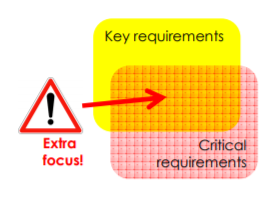
\includegraphics{images/requirements.png}
	\label{fig:exigences}
\end{figure}		

Ci-dessous vous trouverez les exigences nécessaires pour répondre au mieux aux objectifs établis par le commanditaire:

\emph{Exigences critiques:}
\begin{itemize}
\item Être open source
\item Analyser le contenu sémantique d'un document
\item Inscrire dans les documents une appartenance taxonomique établie par la Préfecture
\end{itemize}


\emph{Exigences clés:}
\begin{itemize}
\item Retrouver le nom des partis prenantes dans le document
\item Trouver les dates clefs dans le document (date de rédaction, date de validation, \ldots)
\item Retrouver les arrêtés mentionnées dans le document
\item Permettre la recherche d'un document par taxonomie
\end{itemize}


Les exigences qui nécessitent une attention supplémentaires sont les suivantes:
\begin{itemize}
\item Être open source
\item Analyser le contenu sémantique d'un document
\item Permettre la recherche d'un document par taxonomie
\end{itemize}




